%%
%% This is file `mcmthesis-demo.tex',
%% generated with the docstrip utility.
%%
%% The original source files were:
%%
%% mcmthesis.dtx  (with options: `demo')
%% !Mode:: "TeX:UTF-8"
%% -----------------------------------
%%
%% This is a generated file.
%%
%% Copyright (C)
%%     2010 -- 2015 by latexstudio
%%     2014 -- 2016 by Liam Huang
%%
%% This work may be distributed and/or modified under the
%% conditions of the LaTeX Project Public License, either version 1.3
%% of this license or (at your option) any later version.
%% The latest version of this license is in
%%   http://www.latex-project.org/lppl.txt
%% and version 1.3 or later is part of all distributions of LaTeX
%% version 2005/12/01 or later.
%%
%% This work has the LPPL maintenance status `maintained'.
%%
%% The Current Maintainer of this work is Liam Huang.
%%
\documentclass{mcmthesis}
\mcmsetup{CTeX = true,   % 使用 CTeX 套装时,设置为 true
        tcn = 1911507, problem = B,
        sheet = true, titleinsheet = true, keywordsinsheet = true,
        titlepage = false, abstract = true}
\usepackage{palatino}
\usepackage{lipsum}
\title{Send in the Drones: Developing an Aerial Disaster Relief Response System}
\author{\small \href{http://www.latexstudio.net/}
  {
\includegraphics[width=7cm]{mcmthesis-logo}}}
\date{\today}
\usepackage{geometry}
\geometry{a4paper,left=2.6cm,right=2.6cm,top=3cm,bottom=3cm}
\begin{document}
\begin{abstract}
This article gives an modified integer programming model based on a combination of traditional branch-and-bound method and simulated annealing bin-packing algorithm. It aims at addressing the complicated resource allocation problem, which naturally occurs in designing disaster relief response system, step by step from the perspective of a overall and comprehensive analysis of the interaction within a complex system. 

The DroneGo disaster response system is dispatched to Puerto Rico for two major missons: medical supply delivery and video reconnaissance of road networks, none of which is dispensable. Since focusing on the former solely helps attain a clear insight into this sophisticated problem, we first construct an integer programming model as a basis to be perfected gradually. This model is capable of deciding the cargo container packing configuration, the drone payload packing configurations and the destination of each drones for the demand of the five selected location. Then we extend our analysis to an integrated model for double objectives. In order to specify the appropriate locations of containers and the schedule of drone fleet, we abstract a network from the real map first with the help of geographic information technology. Then we implement the Dijkstra's algorithm to solve for the shortest path as a preparation for drone route planning. Finally we manage to connect our integer programming model with a comlpex network and make a complete model which can solves all the variables which is necessary to establish the DroneGo disaster response system. 

To develop more accurate and efficient model, we utilize the simulated annealing algorithm to address the bin-packing problem which are integrated into the traditional branch-and-bound method for integer programming. The last model improves both accuracy and efficiency considerably, epitomizing what we have been dedicated to in this article.
\begin{keywords}
integer programming; simulated annealing algorithm; bin-packing problem
\end{keywords}
\end{abstract}
\maketitle
\tableofcontents
\newpage

\section{Introduction}
\subsection{Problem Background}
Natural disasters often bring huge casualties and economic losses on human society. In 2017, the worst hurricane in nearly a century landed in Puerto Rico, and left almost the entire island without power, and many without running water or cell phone service. Many highways and roads were blocked because of widespread flooding, which brought great difficulties to rescue route planning. Demand for medical supplies was also soaring for some time. \\

\noindent HELP, Inc., one of non-governmental organizations, is planning to design a transportable disaster response system called DroneGo to conduct medical supply delivery and video reconnaissance.

\subsection{Restatement of Problem}

Our task is to design a DroneGo disaster response system to support potential future disaster scenario similar as the Puerto Rico hurricane. Based on the 2017 situation in Puerto Rico, we will: 

\begin{itemize}
	\item Provide the packing configuration for each of no more than three ISO cargo containers to transport the system.
	\item Find the best locations on Puerto Rico to position these cargo containers to realize both medical supply delivery and video reconnaissance.
	\item Design the drone payload packing configurations, delivery routes and schedule to conduct medical supply delivery, and a drone flight plan to realize video reconnaissance of road networks.
\end{itemize}



\section{General Assumptions}
\textbf{Assumption I}: DroneGo disaster response system consists of up to three ISO cargo containers, a DroneGo fleet and some emergency medical packages. 

\noindent The three cargo containers are identical with standard size, designated as Container A, Container B and Container C respectively. The DroneGo fleet is a combination of drones selected from eight types of potential candidates, namely Drone A to Drone H. Only three types of emergency medical packages are available, referred to as MED 1, MED 2, and MED 3.

\noindent\textbf{Assumption II}: DroneGo disaster response system is designed for possible Puerto Rico hurricane disaster. 

\noindent When disasters occurs, a DroneGo fleet and some emergency medical packages will be packed in up to three cargo containers first of all. 

\noindent Next, each cargo container will be transported to one of the 32 populated places, which are represented by yellow square in Attachment 1, to ensure that DroneGo disaster response system can be timely discovered and well operated. 

\noindent Then both drones and medical packages will be taken out of the containers, and afterwards the latter will be packed into the drone cargo bay that is in fixed connection with the drone. 

\noindent Finally, all drones will depart from the up to three container locations and fly along the main roads on schedule. As is shown in Attachment 1, these main roads connect 32 populated places and make a road network. It is worth pointing out that there are two possible situations for these drones. If the drone carries a cargo bay with medical packages in it, the drone must fly via at least one of five locations in need of medical assistance, referred to as five medical nodes: Jajardo, San Pablo, San Juan, Bayamon and Arecibo, for the purpose of offloading its cargo. However, if the drone carries no cargo, any route without deviation of the road network is allowed.

\noindent\textbf{Assumption III}: To capture the essence of the problem and get rid of unnecessary  complexity, some simplifications have been made. We assume that each drone can deliver medical supplies to at most one location demanding assistance. If two drones from the same container have the same types, they also have the same payload packing configuration.

\section{Symbols and definitions}\label{section:Sym}
\renewcommand\arraystretch{1.5}
\begin{tabular}{ll}
	\hline
	Symbol&  Definition\\
	\hline
	$X$& The number of the containers $X$.\\
	
	$Y$& The number of the containers $Y$.\\
	
	$Z$& The number of the containers $Z$.\\
	
	$X_\alpha$& The number of the drones $\alpha$ packed in the container $X$.\\
	
	$Y_\alpha$& The number of the drones $\alpha$ packed in the container $Y$.\\
	
	$Z_\alpha$& The number of the drones $\alpha$ packed in the container $Z$.\\
	
	$X_{\alpha ij}$& The number of the MED $i$ transported by drone $\alpha$ from\\	 
	& container $X$'s location to the demand location $j$, where $\alpha=A,\cdots,H$,\\ 
	& $i=1,2,3$, $j=1,2,\cdots,5$.\\
	
	$Y_{\alpha ij}$& The number of the MED $i$ transported by drone $\alpha$ from \\
	&container $Y$'s location to the demand location $j$, where $\alpha=A,\cdots,H$,\\
	& $i=1,2,3$, $j=1,2,\cdots,5$.\\
	
	$Z_{\alpha ij}$& The number of the MED $i$ transported by drone $\alpha$ from \\
	&container $Z$'s location to the demand location $j$, where $\alpha=A,\cdots,H$,\\ 
	&$i=1,2,3$, $j=1,2,\cdots,5$.\\
	
	$c_i$& The cost of MED $i$, where $i=1,2,3$.\\
	
	$C_\alpha$& The cost of Drone $\alpha$, where $\alpha=A,B,\cdots,H$.\\
	
	 $W$& The cost of the container.\\
	
	 $V_\alpha$& The volume of the drone $\alpha$, where $\alpha=A,B,\cdots,H$.\\
	
	 $v_i$& The volume of the medical package $i$, where $i=1,2,3$.\\
	
	 $P_\alpha$& The max payload capability of the drone $\alpha$, where $\alpha=A,B,\cdots,H$.\\
	
	 $d$& The supporting days for the medical package demand of all 5 locations.\\
	
	 $M$& A sufficiently large number for big-$M$ method in integer programming.\\ 
	\hline
\end{tabular}


\begin{tabular}{ll}
	\hline
	Symbol&  Definition\\
	\hline	 
	 $\lambda$& A parameter indicating the significance of the video reconnaissance of\\
	 & road networks compared to medical supply delivery. \\
	 
	 $l_\alpha$& The max flight distance of the drone $\alpha$.\\
	 
	 $L$& The total flight distance \\
	 
	 $T$& The number of the nodes in the network of roads.\\
	 
	 $U_{Xm}$& $U_{Xm}=1$ if container $X$ is located at node $m$, where $m=1,2,\cdots,T$.\\ & Otherwise $U_{Xm}=0$.\\
	 
	 $U_{Ym}$& $U_{Ym}=1$ if container $Y$ is located at node $m$, where $m=1,2,\cdots,T$.\\ &Otherwise $U_{Ym}=0$.\\
	 
	 $U_{Xm}$& $U_{Zm}=1$ if container $Z$ is located at node $m$, where $m=1,2,\cdots,T$.\\ &Otherwise $U_{Zm}=0$.\\
	 
	$f(m,j)$& The length of the shortest path from node $m$ to node $j$.\\
	\hline
\end{tabular}

\section{Integer programming model for single objective}\label{section:ip}

The DroneGo disaster response system is sent to Puerto Rico for two major missons: medical supply delivery and video reconnaissance of road networks, none of which is dispensable. Nevertheless, to start with, focusing on the former solely helps attain a clear insight into this sophisticated problem. That leads to our integer programming model.

\subsection{Analysis and assumptions}

\noindent Now assume that the response system are only for medical supply delivery and that the location of each container is so close to its destination that each drone can reach it before the power supply runs out. According to the requirement, the response system must meet the daily medical package demand of the five selected locations in Puerto Rico. Therefore, a natural objective is to maximize the so-called supporting days $d$. Suppose that the amount of the medical packages provided by the Drone fleet can serve location $j$ $(j=1,2,\cdots,5)$ for $d_j$ days. Then the supporting days is defined as
\begin{equation*}
	d=\min\{d_1,d_2,d_3,d_4,d_5\}.
\end{equation*}
For the sake of the optimization of $d$, a lot of independent variables need to be specified appropriately. Firstly, we need to specify the number of the containers transported to the disaster area. We introduce binary variables $X$, $Y$, $Z$ to indicate whether the corresponding cargo container is utilized respectively. Secondly, we have to decide the packing configuration for each container in use. Given the definition of $X_\alpha$ and $X_{\alpha ij}$ in section \ref{section:Sym}, the number of each item to be packed into container $X$ (8 types of drones: Drone A to Drone H; 3 types of medical packages: MED1, MED2, MED3) can be expressed as
 
\begin{equation*}
	X_A,\cdots,X_H,\sum_{\alpha=A}^H\sum_{j=1}^{5}X_{\alpha 1j},\sum_{\alpha=A}^H\sum_{j=1}^{5}X_{\alpha 2j},\sum_{\alpha=A}^H\sum_{j=1}^{5}X_{\alpha 3j}
\end{equation*} 
respectively. Likewise, we can choose values for $Y_\alpha,Y_{\alpha ij}$ and $Z_{\alpha},Z_{\alpha ij}$ to give the packing configuration for the container $Y$ and the container $Z$ respectively. Thirdly, we have to decide the drone payload packing configurations, or alternatively how the medical packages are packed into the drone cargo bay. The number of each type of medical package to be packed into the drone $\alpha$ can be expressed as
\begin{equation*}
\sum_{j=1}^{5}X_{\alpha 1j},\sum_{j=1}^{5}X_{\alpha 2j},\sum_{j=1}^{5}X_{\alpha 3j}
\end{equation*} Finally, the destination of each drone should be given. That is exactly what the variables $X_{\alpha ij},Y_{\alpha ij},Z_{\alpha ij}$ indicate. 

\noindent In a word, we need to adjust the 387 variables
\[
X,Y,Z,X_{\alpha},Y_{\alpha},Z_{\alpha},X_{\alpha ij},Y_{\alpha ij},Z_{\alpha ij}\quad(\alpha=A,\cdots,H;i=1,2,3;j=1,\cdots,5)
\]
for the maximization of $d$.

\subsection{Formalization}

\noindent By imposing proper constraints we obtain the following integer programming problem

\[
\begin{aligned}
\max\quad d
\end{aligned}
\]
\[
\begin{aligned}
\text{s.t.}
\left\{
\begin{array}{lr}
\sum\limits_{i=1}^{3}\sum\limits_{j=1}^{5}v_{i}X_{\alpha ij}\le 8\times 10\times 14\ \text{ if }\alpha=A,B,D &(1)\\
\sum\limits_{i=1}^{3}\sum\limits_{j=1}^{5}v_{i}X_{\alpha ij}\le 24\times 20\times 20\ \text{ if }\alpha=C,E,F,G &(2)\\
\sum\limits_{i=1}^{3}\sum\limits_{j=1}^{5}v_{i}Y_{\alpha ij}\le 8\times 10\times 14\ \text{ if }\alpha=A,B,D &(3)\\
\sum\limits_{i=1}^{3}\sum\limits_{j=1}^{5}v_{i}Y_{\alpha ij}\le 24\times 20\times 20\ \text{ if }\alpha=C,E,F,G &(4)\\
\sum\limits_{i=1}^{3}\sum\limits_{j=1}^{5}v_{i}Z_{\alpha ij}\le 8\times 10\times 14\ \text{ if }\alpha=A,B,D &(5)\\
\sum\limits_{i=1}^{3}\sum\limits_{j=1}^{5}v_{i}Z_{\alpha ij}\le 24\times 20\times 20\ \text{ if }\alpha=C,E,F,G &(6)\\
\sum\limits_{\alpha=A}^{H}V_{\alpha}X_{\alpha}+\sum\limits_{\alpha=A}^{H}\sum\limits_{i=1}^{3}\sum\limits_{j=1}^{5}v_{i}X_{\alpha ij}\le 231\times92\times 94&(7)\\
\sum\limits_{\alpha=A}^{H}V_{\alpha}Y_{\alpha}+\sum\limits_{\alpha=A}^{H}\sum\limits_{i=1}^{3}\sum\limits_{j=1}^{5}v_{i}Y_{\alpha ij}\le 231\times92\times 94&(8)\\
\sum\limits_{\alpha=A}^{H}V_{\alpha}Z_{\alpha}+\sum\limits_{\alpha=A}^{H}\sum\limits_{i=1}^{3}\sum\limits_{j=1}^{5}v_{i}Z_{\alpha ij}\le 231\times92\times 94&(9)\\
\sum\limits_{i=1}^{3}\sum\limits_{j=1}^{5}X_{\alpha ij}\le M X_{\alpha}\ \text{ for }\alpha=A,B,\cdots, G&(10)\\
\sum\limits_{i=1}^{3}\sum\limits_{j=1}^{5}Y_{\alpha ij}\le M Y_{\alpha}\ \text{ for }\alpha=A,B,\cdots, G&(11)\\
\sum\limits_{i=1}^{3}\sum\limits_{j=1}^{5}Z_{\alpha ij}\le M Z_{\alpha}\ \text{ for }\alpha=A,B,\cdots, G&(12)\\
\sum\limits_{\alpha=A}^{H}X_\alpha\le MX&(13)\\
\sum\limits_{\alpha=A}^{H}Y_\alpha\le MY&(14)\\
\sum\limits_{\alpha=A}^{H}Z_\alpha\le MZ&(15)\\
X\le 1&(16)\\
Y\le 1&(17)\\
Z\le 1&(18)\\
\sum\limits_{j=1}^{5}\left(2X_{\alpha 1 j}+2X_{\alpha 2 j}+3X_{\alpha 3 j}\right)\le P_\alpha\text{ for }\alpha=A,B,\cdots, G&(19)\\
\sum\limits_{j=1}^{5}\left(2Y_{\alpha 1 j}+2Y_{\alpha 2 j}+3Y_{\alpha 3 j}\right)\le P_\alpha\text{ for }\alpha=A,B,\cdots, G&(20)\\
\sum\limits_{j=1}^{5}\left(2Z_{\alpha 1 j}+2Z_{\alpha 2 j}+3Z_{\alpha 3 j}\right)\le P_\alpha\text{ for }\alpha=A,B,\cdots, G&(21)\\
\end{array}
\right.
\end{aligned}
\]
\[
\begin{aligned}
\text{s.t.}&
\left\{
\begin{array}{lr}
\sum\limits_{\alpha=A}^{H}(X_{\alpha 11}+Y_{\alpha 11}+Z_{\alpha 11})\ge d&(22)\\
\sum\limits_{\alpha=A}^{H}(X_{\alpha 31}+Y_{\alpha 31}+Z_{\alpha 31})\ge d&(23)\\
\sum\limits_{\alpha=A}^{H}(X_{\alpha 12}+Y_{\alpha 12}+Z_{\alpha 12})\ge 2d&(24)\\
\sum\limits_{\alpha=A}^{H}(X_{\alpha 32}+Y_{\alpha 32}+Z_{\alpha 32})\ge d&(25)\\
\sum\limits_{\alpha=A}^{H}(X_{\alpha 13}+Y_{\alpha 13}+Z_{\alpha 13})\ge d&(26)\\
\sum\limits_{\alpha=A}^{H}(X_{\alpha 23}+Y_{\alpha 23}+Z_{\alpha 23})\ge d&(27)\\
\sum\limits_{\alpha=A}^{H}(X_{\alpha 14}+Y_{\alpha 14}+Z_{\alpha 14})\ge 2d&(28)\\
\sum\limits_{\alpha=A}^{H}(X_{\alpha 24}+Y_{\alpha 24}+Z_{\alpha 24})\ge d&(29)\\
\sum\limits_{\alpha=A}^{H}(X_{\alpha 34}+Y_{\alpha 34}+Z_{\alpha 34})\ge 2d&(30)\\
\sum\limits_{\alpha=A}^{H}(X_{\alpha 15}+Y_{\alpha 15}+Z_{\alpha 15})\ge d&(31)\\
X,Y,Z,X_\alpha,Y_\alpha,Z_\alpha,X_{\alpha ij},Y_{\alpha ij},Z_{\alpha ij} \text{ are nonnegative integers.}&(32)

\end{array}
\right.
\end{aligned}
\]

\subsection{Interpretation}


\noindent Then we will explicitly explain the implications of all the constrains. Constrains (1)-(6) which characterize the volume inequalities are necessary but not sufficient conditions for medical packages to be totally packed into the drone cargo bays. We dispose of the bin packing problem for the time being, since the calculation can be considerably simplified in this way. Similarly, Constrains (7)-(9) are necessary but not sufficient conditions for drones and medical packages to be packed into the containers successfully. Since $M$ is a sufficiently large positive number, constrains (10)-(12) will be activated if only if $X_\alpha$, $Y_\alpha$ or $Z_\alpha$ equal 0. Hence it is impossible for unused drone cargo bays to be loaded any goods in. Likewise, Constrains (13)-(15) can avoid packing items in a unused container. Constrains (16)-(18) indicates that $X$, $Y$ and $Z$ are binary variables. Constraints (19)-(21) exclude the case that the weight of medical packages exceeds the max payload capability of the drone. Constrains (22)-(31) assures that the medical package demand can be satisfied for the first $d$ days at least. Constrain (32) is just a standard condition in any integer programing problem. 

\subsection{Variation}

\noindent If we take the cost of containers, drones and medical packages into consideration and fix the value of $d$, minimizing the total cost also makes sense. To address the minimization problem, we only need to transform the objective function into the following form while all original constraints (1)-(32) still hold:
\[
\begin{aligned}
&\min\quad\sum_{\alpha=A}^{H}\sum_{i=1}^{3}\sum_{j=1}^{5}c_{i}\left(X_{\alpha ij}+Y_{\alpha ij}+Z_{\alpha ij}\right)
+\sum_{\alpha=A}^{H}C_{{\alpha}}\left(X_{\alpha}+Y_{\alpha }+Z_{\alpha }\right)+W(X+Y+Z).
\end{aligned}
\]



\section{Integrated model for double objectives}
Now it is time to extend our analysis to the complete case that both medical supply delivery and video reconnaissance of road networks need to be carried out.

\subsection{Road Network Detection}
To decide the best locations of cargo containers and make a drone flight plan to realize video reconnaissance of road networks, we are supposed to add road network information to the model.     
\begin{figure}[h]
	\small
	\centering
	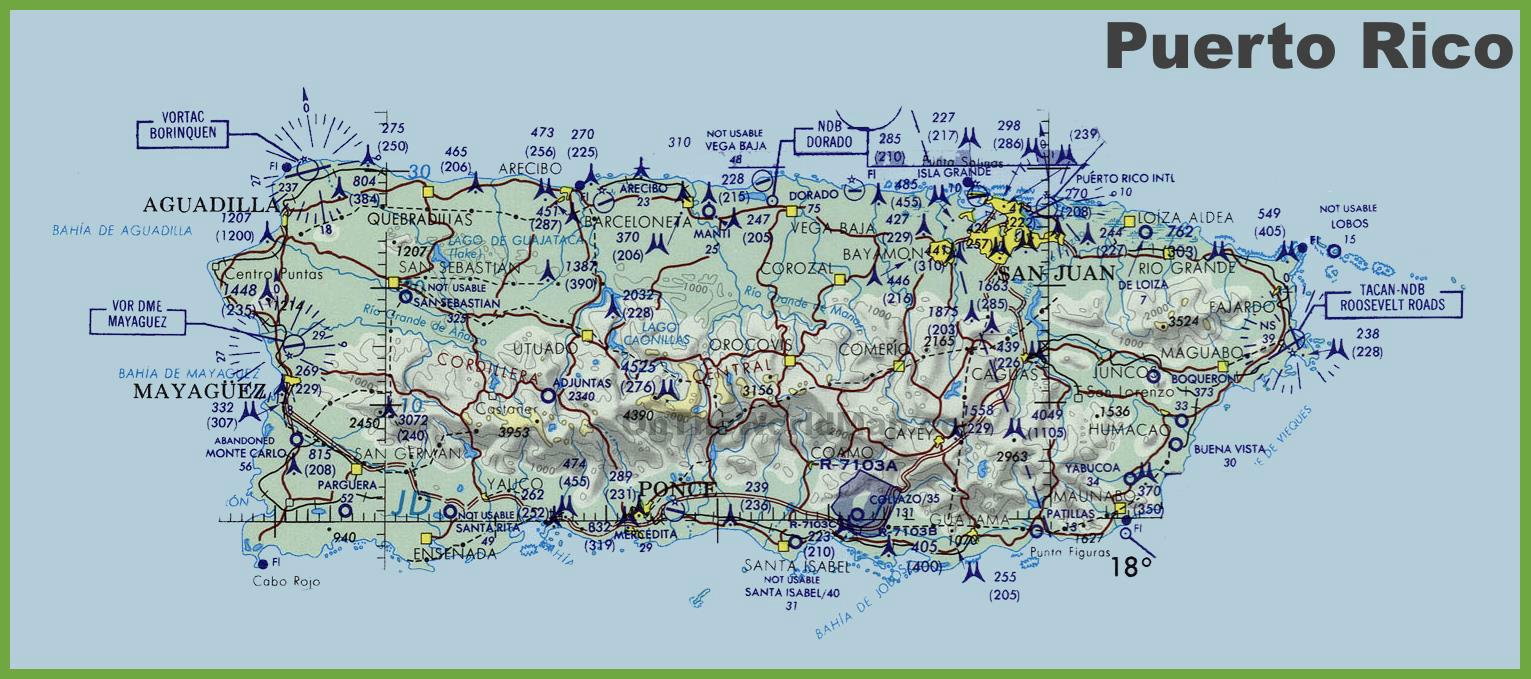
\includegraphics[width=15cm]{1.jpg}
	\caption{Map of Puerto Rico} \label{fig:Map of Puerto Rico}
\end{figure}\\
Based on the following map (Figure 1) provided in Attachments, we use AutoCAD to extract the regional road network of Puerto Rico. The results of road network extraction are shown in Figure 2. 
\begin{figure}[h]
	\small
	\centering
	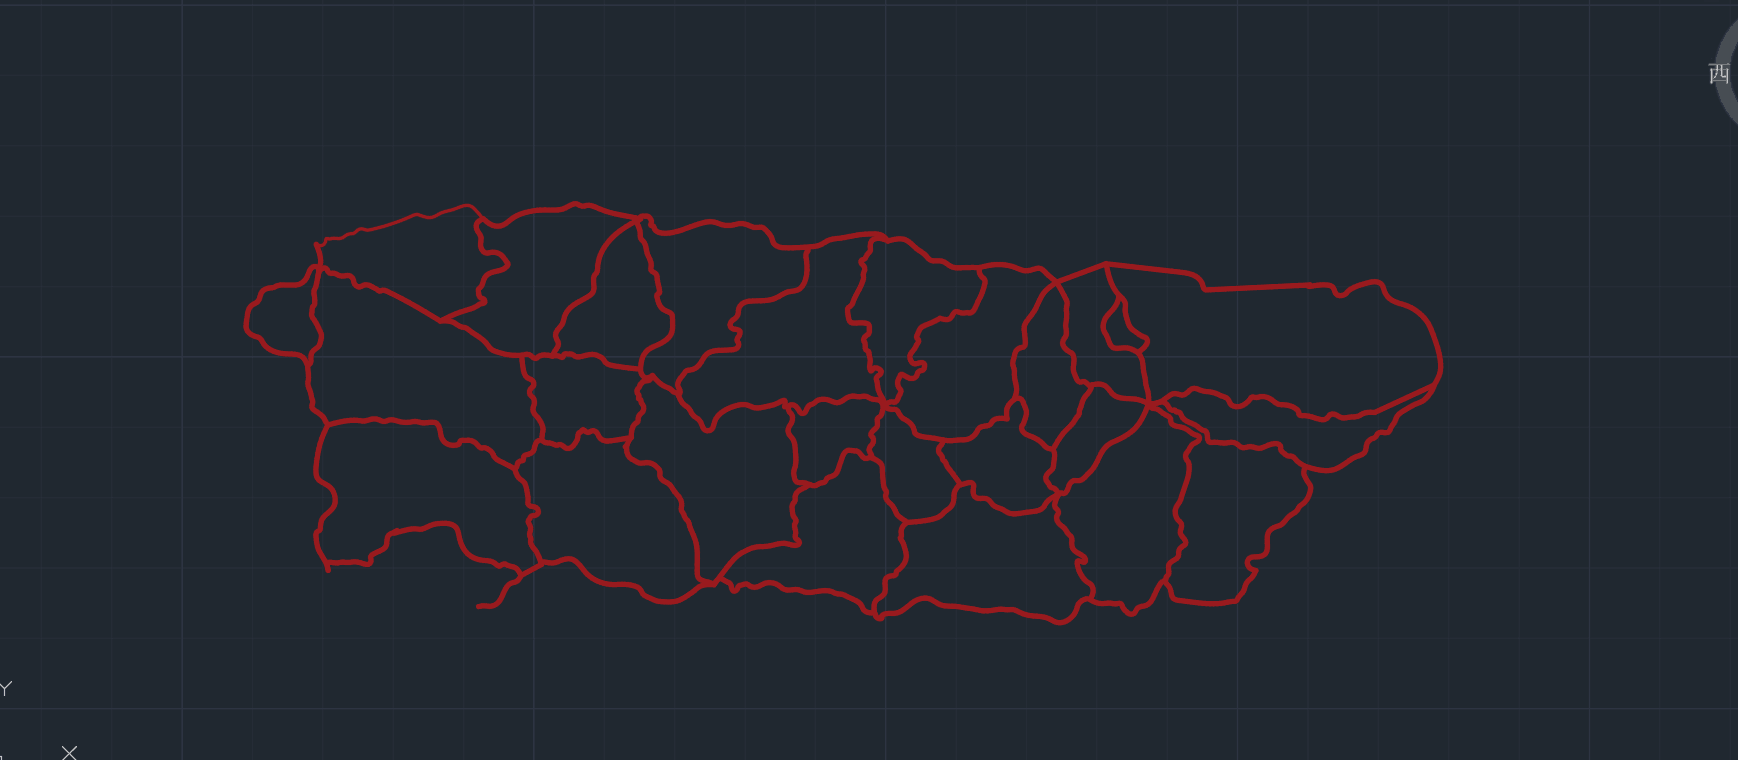
\includegraphics[width=15cm]{8.png}
	\caption{Road Network} \label{fig:2}
\end{figure}

%\subsubsection{Road Network Topology}
\noindent For simplification, we use matrix to represent the topological structure of road network. As shown in the figure 2 below, a simple road network can be represented as a four-dimensional matrix. 
\begin{figure}[h]
	\small
	\centering
	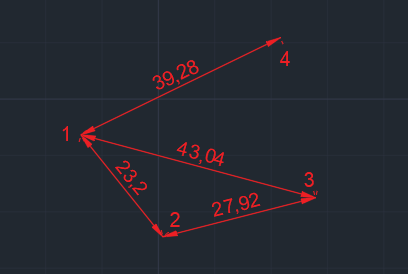
\includegraphics[width=10cm]{9.png}
	\caption{Simple Road Network} \label{fig:4}
\end{figure}
\[
\begin{pmatrix}
{0} & {23.2 } & {43.04 }& {39.28 }  \\
{23.2 } & {0 } & {27.92 } & {-1 } \\
{43.04 } & {27.92  } & {0 } & {-1 } \\
{39.28 } & {-1  } & {-1 } & {0 } \\
\end{pmatrix} 
\]
Similarly, the actual road map shown below, can be expressed as a 32-dimensional matrix. Note that nodes numbered from 1 to 5 in the figure 4 represent hospitals, we just call them medical nodes. And other nodes are mainly populated residential areas, which can be named as normal nodes. 
\begin{figure}[h]
	\small
	\centering
	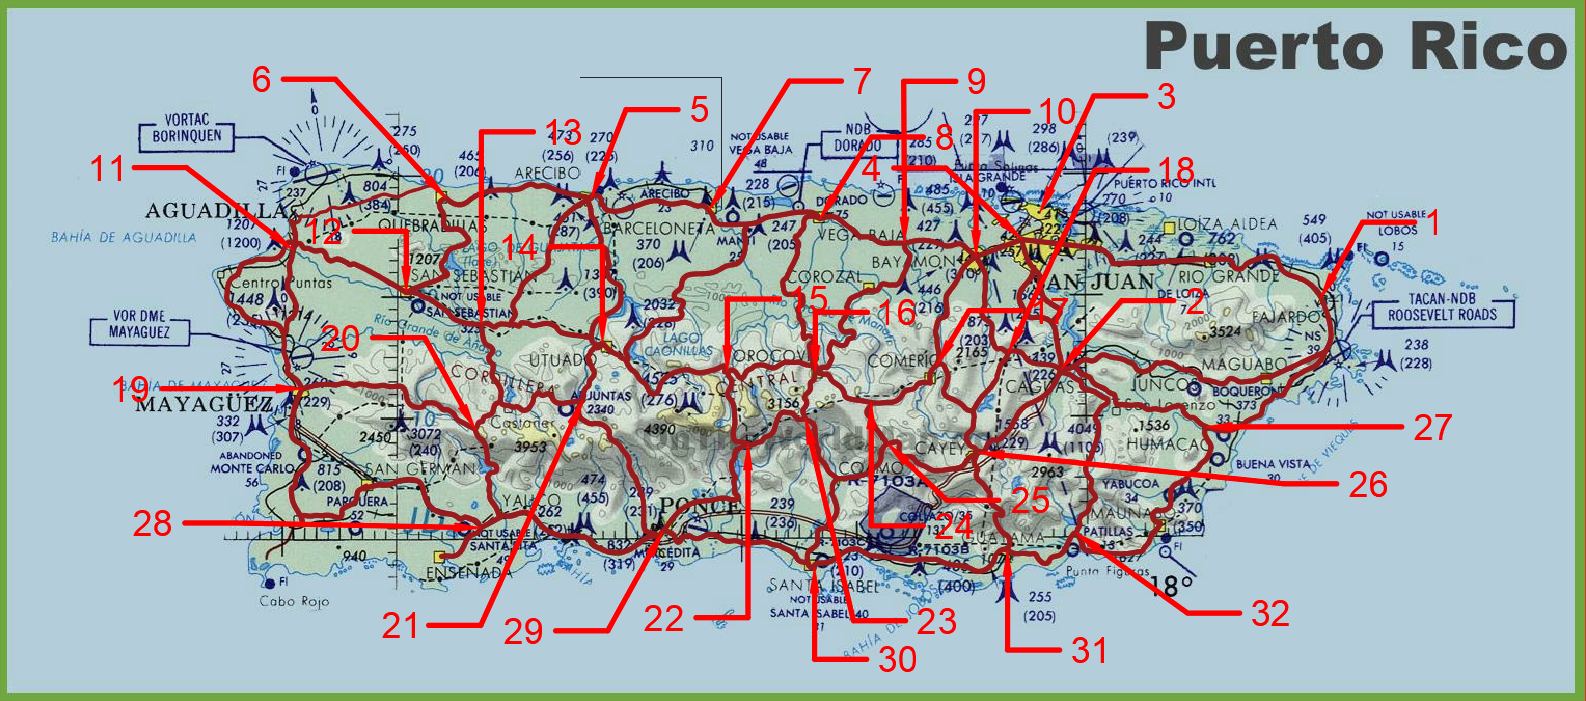
\includegraphics[width=15cm]{6.png}
	\caption{Actual Road Network} \label{fig:4}
\end{figure}



\subsection{Analysis and assumptions}
 Since the variable $d$ named supporting days has been shown to be a reasonable measure of the effect of medical supply delivery, developing some appropriate measures of the effect of video reconnaissance is our priority.

\noindent Assume that drones cannot be recharged, which implies each drone will fly along the road network until its batter is discharged. Another assumption is the max flight distance of the drone is unrelated to the weight of its carrying cargo. When the number of drones is rather large, it is totally reasonable to assume that under no circumstances will any two drones fly abreast along a same road. Thus the sum of flight distances of all the drones can well measure the effect of video reconnaissance. Note that Drone F is not capable of recording video. We can deduce the total flight distance
\[
L=\sum_{\substack{\alpha=A\\ \alpha\ne F}}^{G}l_\alpha (X_\alpha+Y_\alpha+Z_\alpha).
\]
There are several methods of multiobjective optimization. Here we choose a simple linear weighing method in order to obtain a integer programming model. Let $\lambda$ be the weight indicating the significance of the video reconnaissance of road networks compared to medical supply delivery. Then we need to manipulate variables to maximize the weighted measure
\[
d+\lambda L,
\] 
which can be interpreted as the total effect or total utility. 
Besides the 9 variables
\[
X,Y,Z,X_{\alpha},Y_{\alpha},Z_{\alpha},X_{\alpha ij},Y_{\alpha ij},Z_{\alpha ij}
\]
considered in the integer programming model for single objective, more variables are required to describe the location of the container $X$, $Y$, and $Z$, or more specifically, to describe which node  every container should be sent to given the network of roads. Therefore, we resort to binary variables $U_{Xm}$, $U_{Ym}$, $U_{Zm}$ to indicate whether each of containers $X$, $Y$, $Z$ is located at node $m$ respectively. To sum up, we are to specify the following 483 variables
\begin{align*}
	&X,Y,Z,X_{\alpha},Y_{\alpha},Z_{\alpha},X_{\alpha ij},Y_{\alpha ij},Z_{\alpha ij},U_{Xm},U_{Ym},U_{Zm}\\
	&(\alpha=A,\cdots,H;i=1,2,3;j=1,\cdots,5;m=1,\cdots,32)
\end{align*}
to maximize $d+\lambda L$.

\noindent Note that there is no need to introduce any other variables to characterize the flight schedule of the Drone fleet. Instead, as a variety of flight paths lead to the same total flight distance, flight schedule can be specified by simple rules. If a drone carries the medical packages to be transported to node $i$, it will first leave for node $i$ along the shortest path and then fly along an arbitrary major road. If a drone carries no medical packages, it can choose its path from all main roads freely.

\subsection{Formalization}
The objective function of this model is shown as follows:
\[
\begin{aligned}
\max\quad d+\lambda\sum_{\substack{\alpha=A\\ \alpha\ne F}}^{G}l_\alpha (X_\alpha+Y_\alpha+Z_\alpha)
\end{aligned}
\]
In additional to the constraints (1)-(32) introduced in section \ref{section:ip}, new constraints (33)-(39) must hold in the maximization problem. 
\[
\begin{aligned}
\text{s.t.}&
\left\{
\begin{array}{lr}
\sum\limits_{m=1}^{T}U_{Xm}= X&(33)\\
\sum\limits_{m=1}^{T}U_{Ym}= Y&(34)\\
\sum\limits_{m=1}^{T}U_{Zm}= Z&(35)\\
\sum\limits_{i=1}^3X_{\alpha ij}\le M(1-U_{Xm})\quad\text{ if }l_{\alpha}< f(m,j) ,\\\qquad\text{ for }\alpha=A,\cdots,G,m=1,\cdots,T,j=1,\cdots,5&(36)\\
\sum\limits_{i=1}^3Y_{\alpha ij}\le M(1-U_{Ym})\quad\text{ if }l_{\alpha}< f(m,j)  ,\\\qquad\text{ for }\alpha=A,\cdots,G,m=1,\cdots,T,j=1,\cdots,5&(37)\\
\sum\limits_{i=1}^3Z_{\alpha ij}\le M(1-U_{Zm})\quad\text{ if }l_{\alpha}< f(m,j)  ,\\\qquad\text{ for }\alpha=A,\cdots,G,m=1,\cdots,T,j=1,\cdots,5&(38)\\
U_{Xm},U_{Ym},U_{Zm} \in \{0,1\},\ m=1,\cdots,T&(39)
\end{array}
\right.
\end{aligned}
\]
\subsection{Interpretation}
What is left to interpret is the implication of the constrains (33)-(39). Constrain (33) ensures that the variables $U_{Xm}$ are consistent with $X$. In other words, if the container $X$ is utilized, it has to be transported to exact one node of the network. In contrast, if the container $X$ is not in use, it is expected to be placed nowhere. Constrains (34)-(35) are saying the same thing. 

\noindent The constrains (36)-(38) is designed to avoid such cases where some drones carrying medical packages run out of power before reaching their destinations. If the longest flight distance of a drone $l_{\alpha}$ is still less than the shortest distance from its own location to the target medical node, it is not allowed to deliver any cargo at all.

\noindent The constraint (39) is trivial.
\subsection{Variation}
Just by replacing the objective function yields the corresponding cost minimization problem
\[
\begin{aligned}
\min\quad&\sum_{\alpha=A}^{H}\sum_{i=1}^{3}\sum_{j=1}^{5}c_{i}\left(X_{\alpha ij}+Y_{\alpha ij}+Z_{\alpha ij}\right)
+\sum_{\alpha=A}^{H}C_{{\alpha}}\left(X_{\alpha}+Y_{\alpha }+Z_{\alpha }\right)+W(X+Y+Z)\\
&-\lambda\sum_{\substack{\alpha=A\\ \alpha\ne F}}^{G}l_\alpha (X_\alpha+Y_\alpha+Z_\alpha),
\end{aligned}
\]
while all constraints (1)-(39) must hold.


\section{Modified model based on bin-packing algorithm}

In this section we are to resolve a major defect in our previous models. We have been supposing that various items can be packed into a bin if the total volume of all items is not greater than the interior volume of the bin. However, 3D bin-packing simulation software illustrates that in most cases cuboid goods can only occupy 70\%-90\% of the interior space of the bin. Thus our modified model based on advanced 3D bin-packing algorithm is brought forward to reduce the inaccuracy caused by simple volume constraints in integer programming.

%\subsection{Integer programming bin-packing algorithm}
%$s _ { i j } + u _ { i j } + b _ { i j } = 1 \)
%\( \delta _ { i 1 } + \delta _ { i 2 } + \delta _ { i 3 } + \delta _ { i 4 } + \delta _ { i 5 } + \delta _ { i 6 } = 1 \)
%\( x _ { i } - x _ { j } + L \cdot s _ { i j } \leq L - \hat { l } _ { i } \)
%\( y _ { i } - y _ { j } + W \cdot u _ { i j } \leq W - \hat { w } _ { i }$
%$0 \leq x _ { i } \leq L - \hat { l } _ { i } \)
%\( 0 \leq y _ { i } \leq W - \hat { w } _ { i } \)
%\( 0 \leq z _ { i } \leq H - \hat { h } _ { i } \)
%\( \hat { l } _ { i } = \delta _ { i 1 } l _ { i } + \delta _ { i 2 } l _ { i } + \delta _ { i 3 } l _ { i } + \delta _ { i 4 } w _ { i } + \delta _ { i 5 } l _ { i } + \delta _ { i 6 } h _ { i } \)
%\( \hat { w } _ { i } = \delta _ { i 1 } w _ { i } + \delta _ { i 2 } h _ { i } + \delta _ { i 3 } l _ { i } + \delta _ { i 4 } l _ { i } + \delta _ { i 5 } l _ { i } + \delta _ { i 6 } l _ { i } \)
%\( \hat { h } _ { i } = \delta _ { i 1 } h _ { i } + \delta _ { i 2 } w _ { i } + \delta _ { i 3 } h _ { i } + \delta _ { i 4 } l _ { i } + \delta _ { i 5 } w _ { i } + \delta _ { i 6 } l _ { i }$
%$s _ { i j } , u _ { i j } , b _ { i j } \in \{ 0,1 \} \)
%\( \delta _ { i 1 } , \delta _ { i 2 } , \delta _ { i 3 } , \delta _ { i 4 } , \delta _ { i 5 } , \delta _ { i 6 } \in \{ 0,1 \}$
\subsection{Simulated annealing bin-packing algorithm}
\subsubsection{Background}
Simulated annealing arithmetic was formed in the early 1980s. Its idea originated from the annealing process of solids, heating solids to a sufficiently high temperature and then cooling them slowly. When the temperature was raised, the internal energy of particles in solids became disordered and increased, while when the temperature was slowly cooled, the particles gradually became orderly. In theory, if the cooling process was slow enough, then either of them would be cooled. Solids can achieve thermal equilibrium at temperature, and when cooled to low temperature, they will reach the minimum state of internal energy at this low temperature.      

\noindent In this process, it is an important step to achieve thermal equilibrium at any constant temperature. When applying simulated annealing to optimization problems, temperature $T$ can generally be regarded as control parameter, objective function value f as internal energy $E$, and a state of solid at a certain temperature $T$ corresponds to a solution $x$. Then the algorithm tries to reduce the objective function value $f$ (internal energy $E$) gradually with the decrease of the control parameter $T$ until it reaches the global minimum (the lowest energy state in low temperature annealing), just like the solid annealing process.

\subsubsection{Model Assumptions}
\begin{itemize}
	\item The dimensions of the goods are integers.
	\item The goods can only be placed along the coordinate axes of the container, that is, parallel to the edges of the container.
	\item The coordinate system is a three-dimensional Cartesian coordinate system. The length, width and height of the container correspond to the X, Y and Z axes of the Cartesian coordinate system respectively.
	\item $(x, y, z)$ is the coordinate of the lower-left corner of the front side of the container.
	\item In the process of loading, the goods put into the container can move downward, forward and left until its bottom, front and left are adjacent to other goods or containers.
	\item The goods arrive at the same destination.
	\item The extrusion deformation of goods can be neglected.
\end{itemize}

\subsubsection{Simulated annealing Algorithm}
\begin{itemize}
	\item Set the initial annealing temperature $T_0$, and generate an initial solution $x_0$ at random and calculate the corresponding objective function $E(X_0)$.
	\item Make $T$ equal to the next value in the cooling schedule $T_i$.
	\item Pick a random neighbour of the current solution $x_i$, generate a new solution $x_j$, calculate the corresponding objective function value $E(x_j)$, and get $\Delta E=E(x_j)-E(x_i)$.
	\item If  $\Delta E > 0$, the new solution $x_j$ is accepted as the new current solution; otherwise, $x_j$ is accepted with a probability of $exp(-\Delta E/T_i)$. 
	\item Repeat steps 3 and 4 $L_k$ times at temperature $T_i$.
	\item Transfer the algorithm  to step 2 till $T=T_f$.
\end{itemize}

\noindent The algorithm is essentially divided into two layers of cycles, generating new solutions at any temperature random disturbance, and calculating the change of the objective function value to determine whether it is accepted or not. Because the initial temperature of the algorithm is relatively high, the new solution of increasing E may also be accepted at the beginning, so it can jump out of the local minimum, and then by slowly lowering the temperature, the algorithm may eventually converge to the global optimal solution. It is also pointed out that although the acceptance function is very small at low temperature, the possibility of accepting worse solutions is still not excluded. Therefore, the best feasible solution (historical optimal solution) encountered in annealing process is generally recorded and output together with the last accepted solution before terminating the algorithm.

\subsection{Modified model simulated annealing algorithm }

In this section we will modify our normal integer programming model by combining simulated annealing algorithm. 
Consider a general integer programming problem.
\[
\max Z = \sum _ { j = 1 } ^ { n } c _ { j } x _ { j }
\]
s.t.
\[
\sum _ { j = 1 } ^ { n } a _ { i j } x _ { j } \leq b _ { i }\text{ for }i=1,2,\cdots,m
\]
and
\[
x _ { j } \geq 0 , \quad \text { for } j = 1,2 , \cdots , n
\]
\[
x _ { j } \text { is integer, } \quad \text { for } j = 1,2 , \cdots , n .
\]
A common and efficient algorithm for integer programming is branch-and-bound method, which can be summarized as follows:
\begin{enumerate}
	\item[0.] Initialization: Set $Z^*$. Apply the bounding step, fathoming step, and optimality test described below to the whole problem. If not fathomed, classify this problem as the one remaining subproblem for performing the first full
	iteration below.
	Steps for each iteration:
	\item Branching: Among the remaining (unfathomed) subproblems, select the one that was
	created most recently. (Break ties according to which has the larger bound.) Among
	the integer-restricted variables that have a noninteger value in the optimal solution for
	the LP relaxation of the subproblem, choose the first one in the natural ordering of the
	variables to be the branching variable. Let $x_j$ be this variable and $x_j^*$ its value in this solution. Branch from the node for the subproblem to create two new subproblems by adding the respective constraints $x_j\le[x_j^*]$ and $x_j\ge[x_j^*]+1$.
	\item Bounding: For each new subproblem, obtain its bound by applying the simplex method
	(or the dual simplex method when reoptimizing) to its LP relaxation and using the
	value of $Z$ for the resulting optimal solution.
	\item Fathoming: For each new subproblem, apply the three fathoming tests given below, and discard those subproblems that are fathomed by any of the tests.\\
	Test 1: Its bound $Z^*$, where $Z^*$ is the value of $Z$ for the current incumbent.\\
	Test 2: Its LP relaxation has no feasible solutions.\\
	Test 3: The optimal solution for its LP relaxation has integer values for the integerrestricted variables. (If this solution is better than the incumbent, it becomes the new incumbent and test 1 is reapplied to all unfathomed subproblems with	the new larger $Z^*$.)\\
	Optimality test: Stop when there are no remaining subproblems that are not fathomed; the current incumbent is optimal. Otherwise, perform another iteration.
\end{enumerate}

\noindent Now we change the traditional fathoming step to yield a more accurate solution. For given $X_\alpha$ and $X_{\alpha ij}$, we can use the simulated annealing bin-packing algorithm to decide whether it is a possible packing configuration. Thus the original test 2 should be extended. Even though its LP relaxation has feasible solutions, they can be specified as an impossible packing configuration by bin-packing algorithm, which implies fathoming should be conducted. 

\noindent After the simulated annealing bin-packing algorithm is involved, we find the optimal solution in normal integer programming was overwhelmingly large than the actual situation. 

\section{The Model Results}
\lipsum[6]

\section{Validating the Model}
\lipsum[9]

\section{Conclusions}
\lipsum[6]

\section{A Summary}
\lipsum[6]

\section{Evaluate of the Model}

\section{Strengths and weaknesses}
\lipsum[12]

\subsection{Strengths}
\begin{itemize}
\item \textbf{Applies widely}\\
This  system can be used for many types of airplanes, and it also
solves the interference during  the procedure of the boarding
airplane,as described above we can get to the  optimization
boarding time.We also know that all the service is automate.
\item \textbf{Improve the quality of the airport service}\\
Balancing the cost of the cost and the benefit, it will bring in
more convenient  for airport and passengers.It also saves many
human resources for the airline. \item \textbf{}
\end{itemize}

\section*{Memo}
\addcontentsline{toc}{section}{Memo}
$\mathbf{To:}$ Chief Operating Officer \\
$\mathbf{From:}$ Team 1911507\\
$\mathbf{Date:}$ 29 January, 2019\\
$\mathbf{Subject:}$ Suggestions for DroneGo Disaster Response System\\

\noindent We are writting to report our main modeling results and suggestions for  DroneGo disaster response system.\\

\noindent$\mathbf{Modeling}\ \mathbf{Results:}$
\begin{itemize}
	\item 
	\item 
\end{itemize}

\noindent$\mathbf{Recommendations:}$
\begin{itemize}
	\item 
	\item 
\end{itemize}

\noindent We hope that our suggestions are helpful. Please contact us if you have any questions.



\begin{thebibliography}{99}
\bibitem{1} D.~E. KNUTH   The \TeX{}book  the American
Mathematical Society and Addison-Wesley
Publishing Company , 1984-1986.
\bibitem{2}Lamport, Leslie,  \LaTeX{}: `` A Document Preparation System '',
Addison-Wesley Publishing Company, 1986.
\bibitem{3}\url{http://www.latexstudio.net/}
\bibitem{4}\url{http://www.chinatex.org/}
\end{thebibliography}

\begin{appendices}

\section{First appendix}

\lipsum[13]

Here are simulation programmes we used in our model as follow.\\

\textbf{\textcolor[rgb]{0.98,0.00,0.00}{Input matlab source:}}
\lstinputlisting[language=Matlab]{./code/mcmthesis-matlab1.m}

\section{Second appendix}

some more text \textcolor[rgb]{0.98,0.00,0.00}{\textbf{Input C++ source:}}
\lstinputlisting[language=C++]{./code/mcmthesis-sudoku.cpp}

\end{appendices}
\end{document}

%%
%% This work consists of these files mcmthesis.dtx,
%%                                   figures/ and
%%                                   code/,
%% and the derived files             mcmthesis.cls,
%%                                   mcmthesis-demo.tex,
%%                                   README,
%%                                   LICENSE,
%%                                   mcmthesis.pdf and
%%                                   mcmthesis-demo.pdf.
%%
%% End of file `mcmthesis-demo.tex'.
